%% Scandinavian Journal of Medicine & Science in Sports — Original Article — FIRST DRAFT (29 Oct 2026)
%% Vancouver numbered references (unsrt + natbib). Same LaTeX setup as the A1/SMO manuscripts.

\documentclass[12pt,a4paper]{article}

\usepackage[utf8]{inputenc}
\usepackage[T1]{fontenc}
\usepackage{times}
\usepackage[margin=2.5cm]{geometry}
\usepackage{setspace}
\doublespacing

\usepackage{graphicx}
\graphicspath{{../figures/}}
\usepackage{float}
\usepackage{placeins}
\usepackage{amsmath,amssymb}
\usepackage{booktabs}
\usepackage{enumitem}
\usepackage[colorlinks=true,linkcolor=blue,citecolor=blue,urlcolor=blue]{hyperref}
\usepackage[numbers,sort&compress]{natbib}
\usepackage{lineno}
\linenumbers

\begin{document}

% ── Title page ──────────────────────────────────────────────

\begin{titlepage}
\vspace*{2cm}

{\noindent\LARGE\bfseries Does starting age predict who stays? Competition debut and long-term participation in youth track and field\par}

\vspace{1.5cm}

{\noindent\large
Atle G.\ Guttormsen$^{1,*}$ \\
\href{https://orcid.org/0000-0003-0188-8462}{ORCID: 0000-0003-0188-8462}
}

\vspace{0.8cm}

{\noindent
$^1$School of Economics and Business, Norwegian University of Life Sciences (NMBU), Ås, Norway
}

\vspace{0.8cm}

{\noindent
$^*$Corresponding author:\\
Atle G.\ Guttormsen\\
School of Economics and Business\\
Norwegian University of Life Sciences (NMBU)\\
P.O.\ Box 5003, 1432 Ås, Norway\\
E-mail: atle.guttormsen@nmbu.no
}

\vspace{1.5cm}

{\noindent\textbf{Running head:} Debut age and retention in youth athletics}

\vspace{0.5cm}

{\noindent\textbf{Word count:} $\sim$3\,000 (main text, excluding abstract, references, tables, and figure legends)}

\end{titlepage}

% ── Abstract ────────────────────────────────────────────────

\newpage
\section*{Abstract}

\noindent Whether starting competitive sport early harms or protects long-term participation is contested: the early-specialisation literature cautions against early entry, while the largest prospective dropout study found that dropouts had started \emph{later}. No population study has tested the question in an individual sport. Using the Norwegian Athletics Federation's complete competition registry, which is electronically complete from 2011, we followed every athlete born 2001--2005 whose first registered competition occurred at ages 10--16 (n = 17\,496; 50\,\% female) to the end of 2026; 546 (3.1\,\%) were active as seniors (age $\geq$20). Senior conversion was U-shaped in debut age: relative to debut at age 10 (3.8\,\%), adjusted odds were lowest for debuts at 11--14 (OR 0.53--0.75) and highest for debut at 16 (6.6\,\%; OR 1.73, 95\,\% CI 1.15--2.59), with a null linear trend (OR 0.99 per year, 95\,\% CI 0.94--1.04). Measured from their own debut, however, later starters left much faster: five years after debut, 17\,\% of those who started at 10 were still competing against 3--7\,\% of those who started at 12--16, and survival curves with delayed entry converged by about age 16. Among athletes still active at 17, debut age appeared protective (OR 0.87 per year) but the association disappeared once current competition volume was controlled (OR 0.97, 95\,\% CI 0.92--1.03). Neither the claim that early competitive entry undermines retention nor the claim that late entry does was supported. Starting age matters far less than current engagement --- and every entry age produced senior athletes.

\vspace{0.5em}
\noindent\textbf{Keywords:} youth sport; dropout; starting age; early specialisation; athlete retention; registry study; track and field

\newpage

% ════════════════════════════════════════════════════════════
\section{Introduction}

When should children enter competitive sport? The question sits at the centre of the early-specialisation debate, and the two main positions make opposite predictions about participation. One line of argument, prominent in consensus statements, cautions that early competitive engagement risks burnout and withdrawal \cite{difiori2014}; on this view, later entry should protect retention. The opposite prediction comes from the retention literature itself: in the largest prospective dropout study to date, among 1\,762 Dutch football players, those who dropped out had \emph{started organised football later} than those who stayed, and the authors recommended recruiting from early childhood \cite{vanyperen2021}. Direct tests are scarce. Markers of early specialisation failed to predict actual dropout in the one study that measured both \cite{larson2019}, systematic reviews of youth sport dropout identify motivational and social factors rather than starting age \cite{crane2015,espedalen2022}, and the retrospective expertise literature --- which finds that eventual elites often entered their main sport later \cite{barth2022,gullich2025} --- samples on success and therefore cannot speak to population-level retention. No study has followed a complete national entry population of an individual sport and asked what age at entry implies for who is still competing a decade later.

The Norwegian athletics registry permits exactly that design. Every sanctioned result in Norway is registered, the registry is electronically complete from 2011, and competition begins at age 10. For athletes born in 2001 or later, the full competitive career is therefore observed from its first day, with no left truncation: age at first registered competition is measured exactly, for everyone who ever entered, not only for those who later succeeded. Three earlier studies of the same registry frame the present one. Relative-age selection was found to be fully established at the entry stage and stable thereafter, locating the system's selection pressure at the point of entry rather than in adolescent talent identification \cite{guttormsen2026rae}. A 14-year cohort study found that competition volume at ages 13--14 predicted senior retention far better than performance did, and that exit is preceded by behavioural withdrawal \cite{guttormsen2026dropout}. A companion study of performance trajectories found that progression predicts retention beyond volume --- but that, here too, the \emph{recent} window dominates the earlier one \cite{guttormsen2026progression}. Against that background, entry age is the natural next exposure: it is the first behavioural fact the registry records about an athlete.

We pre-specified three questions. \textbf{H1:} among all athletes whose first registered competition fell at ages 10--16, is debut age associated with being active as a senior? The two literatures predict opposite directions, so H1 is two-sided, a U-shape is plausible, and the categorical contrast is the primary display. \textbf{H2:} once started, do later debutants exit faster, as the football findings suggest \cite{vanyperen2021}? \textbf{H3:} among athletes still active at age 17, does entry history add anything beyond current engagement --- or does the registry repeat its now-familiar lesson that current behaviour dominates history \cite{guttormsen2026dropout,guttormsen2026progression}? Interpretation rules were fixed in advance: the exposure is \emph{competition debut}, not the start of sport participation or training, and selection into late debut (already-interested adolescents choosing athletics) is expected and addressed in the design and interpretation. The analysis plan was committed to version control before any exposure--outcome model was estimated; the study was not externally preregistered.

% ════════════════════════════════════════════════════════════
\section{Materials and methods}

\subsection{Data source and design}

The Norwegian Athletics Federation's results database registers every sanctioned competition result in Norway and Norwegian athletes' results abroad. We used a frozen extract of 29 October 2026 (results dated on or before that day). Only participation fields were extracted --- athlete, date, meet, club, approval status; no performance data of any kind were used, in keeping with the Norwegian children's sport regulations, which this study's design renders moot since it needs no marks. Age is calendar-year age (competition year minus birth year), the basis of Norwegian age classes. Reporting follows STROBE \cite{vonelm2007}.

\subsection{Sample}

All athletes born 2001--2008 entered the extraction (n = 33\,666, with 675\,707 result rows; 1\,526 non-approved rows and 116 rows below age 10 were excluded). The 28\,339 athletes with an approved result at age 10 or older constitute the debutant population; 865 without registered sex and 732 (2.6\,\%) whose debut fell at age 17 or later (analysed as a sensitivity category) were excluded from the primary sample. The primary sample comprises the 17\,496 athletes born 2001--2005 whose debut fell at ages 10--16 --- cohorts whose follow-up extends past age 20 for everyone --- of whom 50.1\,\% were female and 546 (3.1\,\%) met the senior-activity outcome. Athletes born 2006--2008 contribute to descriptive analyses of entry patterns only.

\subsection{Exposure, outcomes, and covariates}

The exposure is \emph{debut age}: calendar-year age at the athlete's first approved registered result (10--16), treated categorically (reference: debut at 10) and as a linear trend. The primary outcome, identical to the companion studies \cite{guttormsen2026dropout,guttormsen2026progression}, is \emph{active senior}: at least two approved results in the same calendar year at age 20 or older. Secondary outcomes were at least one result at age $\geq$20, activity at age $\geq$17, and retention $k$ years after debut ($k$ = 1--5, computed only over athlete-years fully observable by 2025). Covariates were sex, birth cohort, region (modal competition district in the debut season), baseline club (modal club in the debut season) with the logarithm of a club-size proxy (study athletes per club), birth quarter where an exact birth date existed, debut-season competition days, and a COVID-19 flag for debuts in 2020--2021.

\subsection{Statistical analysis}

H1 was estimated by logistic regression in the primary sample, with debut age categorical and linear, adjusted for sex, cohort, region, and club size, with club-clustered standard errors as a sensitivity. H2 was addressed two ways, because they answer different forms of the question. First, descriptively on the \emph{duration} clock: the proportion still competing $k$ years after their own debut, by debut age --- the comparison that aligns athletes at the same career stage. Second, on the \emph{age} clock: a Cox model with age as the timescale and delayed entry at debut \cite{anderson1983}, athletes leaving the risk set at their last active age (+0.5) and censored if active in 2025--2026. The age-scale coefficient on debut age compares, at the same age, athletes at different career stages; it therefore blends duration and entry effects, and is reported with that caveat, with the duration-clock table as the primary evidence for H2. H3 was a landmark analysis among athletes active at age 17: senior activity regressed on debut age with sex and cohort, with and without current engagement (competition days at ages 16--17, standardised). Pre-specified robustness analyses excluded COVID-19 debuts, varied the outcome, added debut-season volume, split the cohorts (2001--2003 vs.\ 2004--2005), included debut at 17+ as a category, and explored a debut age $\times$ birth-quarter interaction --- the last on the selected subsample with exact birth dates, since coverage rises steeply with debut age (Table~\ref{tab:char}). Analyses used Python 3.13 (pandas, statsmodels, lifelines).

\subsection{Ethics and transparency}

The data are public competition results; no individual is identified; no performance data were used, and nothing below age 13 beyond participation itself was analysed. As for the companion registry studies, the project falls outside the scope of the Norwegian Health Research Act, and an assessment from Sikt was obtained. The analysis plan, hypotheses, estimands, and interpretation rules were committed to version control before estimation; code and aggregate outputs are available, and athlete-level files are regenerable from the registry.

% ════════════════════════════════════════════════════════════
\section{Results}

\subsection{Who debuts when}

Debut at 10, the first eligible age, was the single most common entry point and its share grew across cohorts (32.6\,\% of debutants born 2001; 43.9\,\% born 2008), but late entry remained substantial: roughly one debutant in six entered at 14 or later (Figure~\ref{fig:cohort}). Table~\ref{tab:char} describes the three debut groups. Late debutants were more often male (female share 52.2\,\% for debut at 10--11 against 42.0\,\% for 14--16). The typical debut was brief in every group: the median debutant competed on a single day in the debut season, and median career length was two seasons for debut at 10--11 and one season otherwise. Exact birth dates --- needed for birth-quarter analyses --- existed for 38.6\,\% of early, 63.8\,\% of mid, and 88.5\,\% of late debutants, the registry's known pattern of missingness concentrating among brief early participants \cite{guttormsen2026rae}; among those with known dates, the familiar first-quarter overrepresentation was present at every debut age (Q1 26--29\,\% against Q4 20--22\,\%).

\begin{table}[H]
\centering
\caption{Characteristics of the primary sample (born 2001--2005, debut at ages 10--16), by debut group.}
\label{tab:char}
\small
\begin{tabular}{lccc}
\toprule
Characteristic & Debut 10--11 & Debut 12--13 & Debut 14--16 \\
\midrule
n & 10\,242 & 4\,220 & 3\,034 \\
Female, \% & 52.2 & 50.8 & 42.0 \\
Exact birth date available, \% & 38.6 & 63.8 & 88.5 \\
Born Q1, \% of those with birth date & 29.2 & 26.1 & 27.1 \\
Born Q4, \% of those with birth date & 19.9 & 21.9 & 19.8 \\
Competition days in debut season, median (IQR) & 1 (1--3) & 1 (1--3) & 1 (1--2) \\
Career length, seasons, median (IQR) & 2 (1--4) & 1 (1--3) & 1 (1--2) \\
Debut season 2020--2021, \% & 0.0 & 0.0 & 6.3 \\
\bottomrule
\end{tabular}
\vspace{0.3em}
\parbox{0.92\textwidth}{\footnotesize By construction, cohorts born 2001--2005 could only experience a 2020--2021 debut at ages 14 and above.}
\end{table}

\begin{figure}[H]
\centering
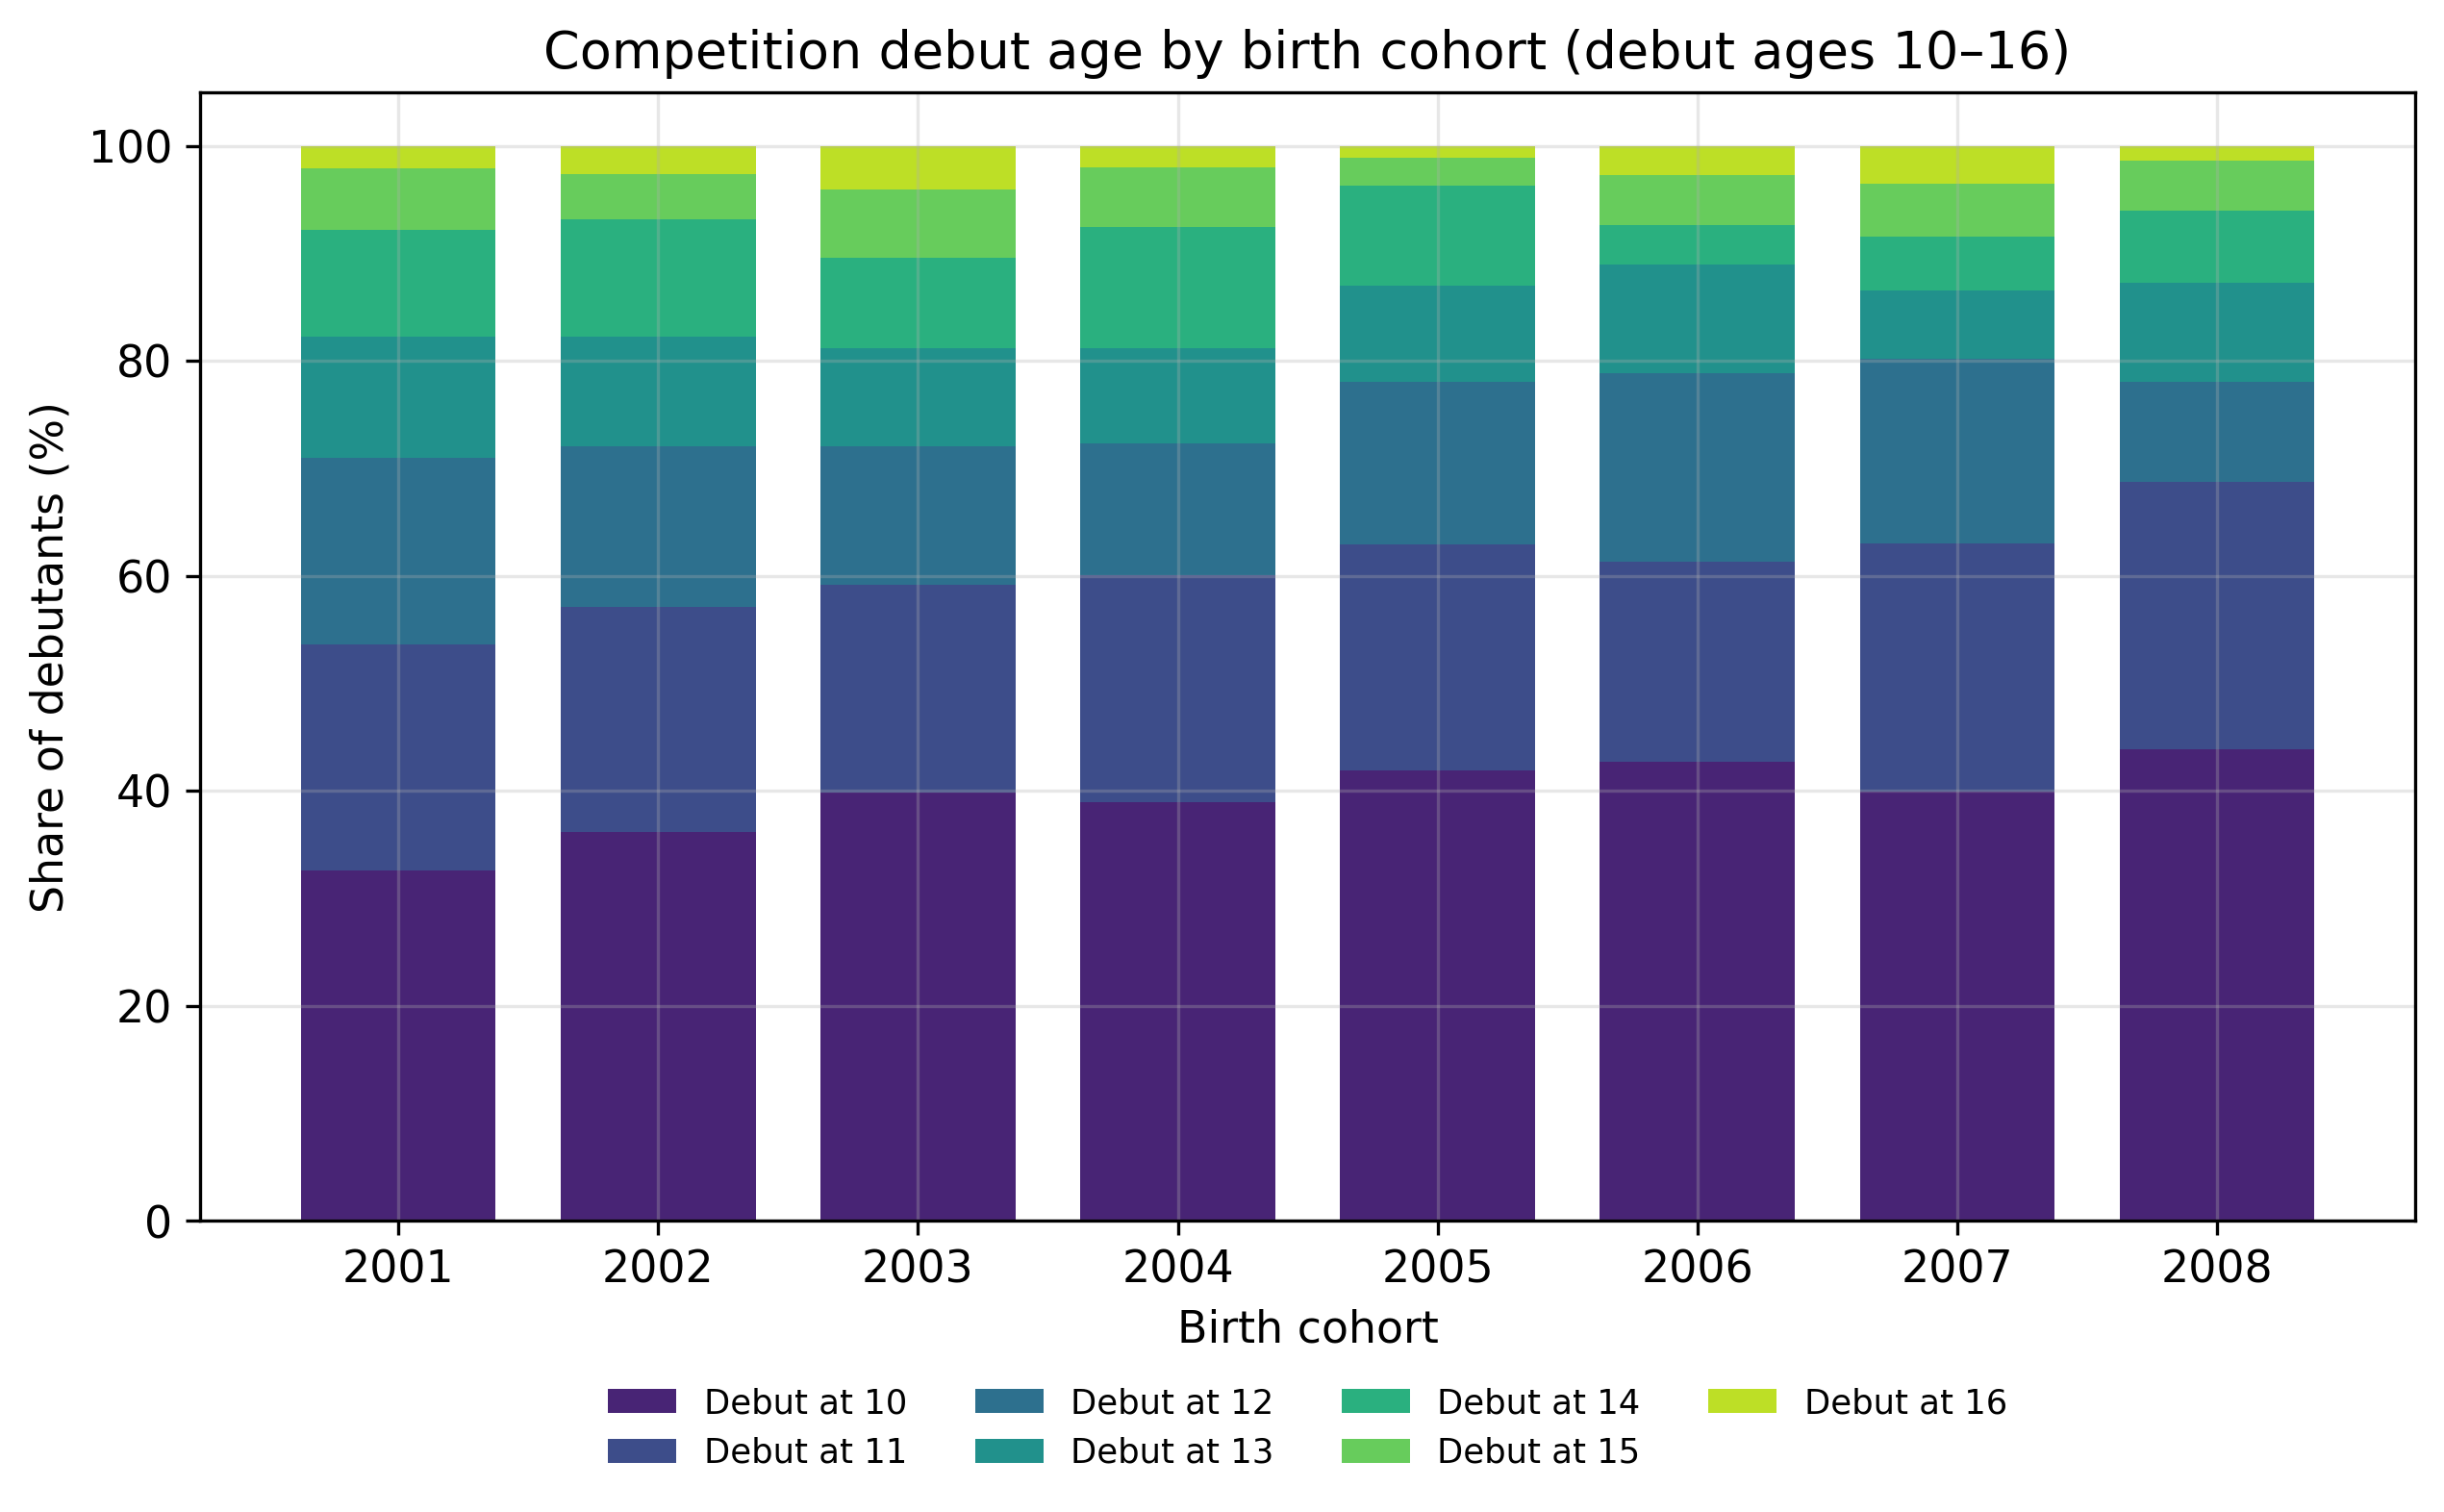
\includegraphics[width=0.85\textwidth]{fig1_debut_age_by_cohort.png}
\caption{Competition debut age by birth cohort (all debutants born 2001--2008, debut ages 10--16).}
\label{fig:cohort}
\end{figure}

\subsection{Senior conversion is U-shaped in debut age (H1)}

Of the 17\,496 debutants, 546 (3.1\,\%) were active as seniors. Conversion was not monotone in debut age (Figure~\ref{fig:ushape}): it was 3.8\,\% for debut at 10 (253/6\,626), fell to 2.0--2.4\,\% for debuts at 11, 12 and 14 (bottom: 2.1\,\% at 12), and rose to 3.9\,\% at 15 and 6.6\,\% at 16 (28/424). Adjusted for sex, cohort, region, and club size (Table~\ref{tab:h1}), debuts at 11--14 had significantly lower odds than debut at 10 (OR 0.53--0.75), debut at 15 the same odds (OR 1.00), and debut at 16 markedly higher odds (OR 1.73, 95\,\% CI 1.15--2.59). The linear trend across 10--16 was correspondingly null (OR 0.99 per year, 95\,\% CI 0.94--1.04) --- a flat average concealing a U. Neither of the two simple hypotheses --- early entry harms, or late entry harms --- fits this shape.

\begin{table}[H]
\centering
\caption{Adjusted odds of senior activity (age $\geq$20) by debut age (n = 17\,496; 546 events). Reference: debut at age 10. Adjusted for sex, birth cohort, region, and club size.}
\label{tab:h1}
\small
\begin{tabular}{lc}
\toprule
Debut age & OR (95\,\% CI) \\
\midrule
10 (reference; raw conversion 3.8\,\%) & 1.00 \\
11 & 0.63 (0.49--0.81) \\
12 & 0.53 (0.39--0.71) \\
13 & 0.75 (0.55--1.02) \\
14 & 0.62 (0.44--0.86) \\
15 & 1.00 (0.70--1.45) \\
16 & 1.73 (1.15--2.59) \\
\midrule
Linear trend, per +1 year of debut age & 0.99 (0.94--1.04) \\
\bottomrule
\end{tabular}
\end{table}

\begin{figure}[H]
\centering
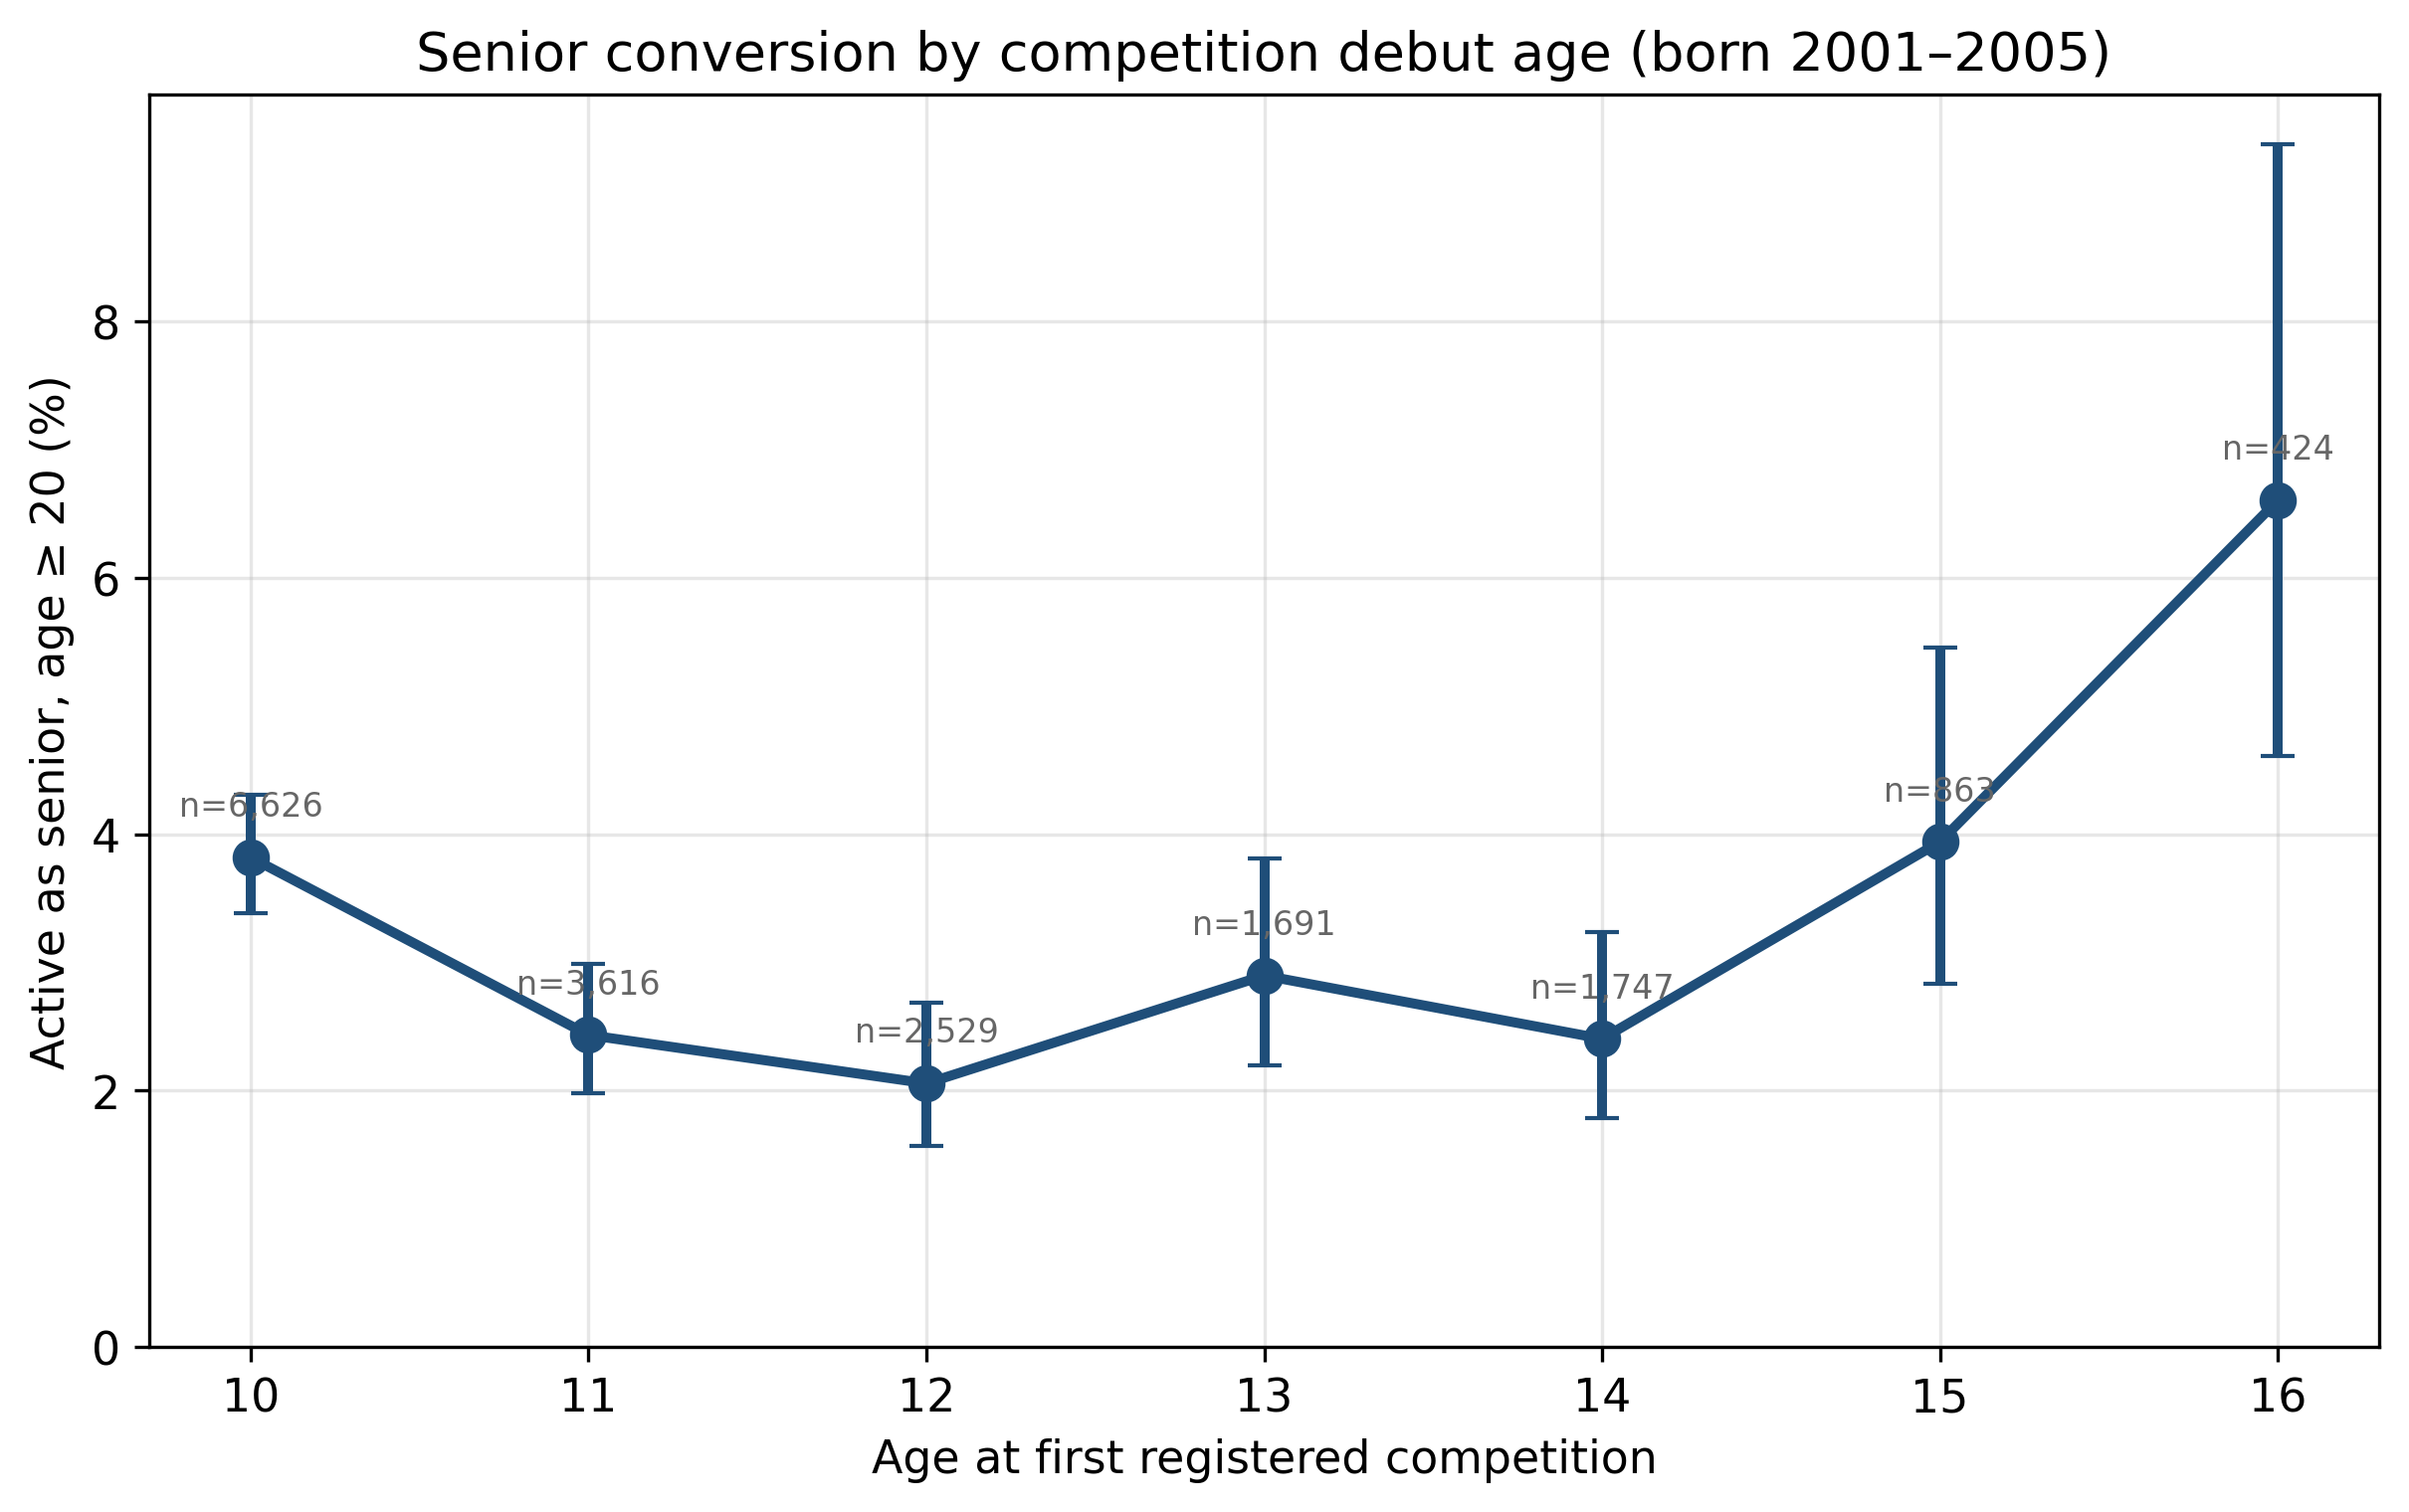
\includegraphics[width=0.85\textwidth]{fig2_senior_by_debut_age.png}
\caption{Senior conversion by competition debut age, with Wilson 95\,\% confidence intervals (born 2001--2005).}
\label{fig:ushape}
\end{figure}

\subsection{Later starters leave faster --- on their own clock (H2)}

Aligned on time since debut (Table~\ref{tab:retention}; Figure~\ref{fig:retk}), early entrants were far more durable. One year after the debut season, 51\,\% of those who debuted at 10 were still competing, against 34--40\,\% of those who debuted at 11--14 and 26\,\% at 15. Five years after debut the gap had widened to 17\,\% against 3--7\,\%. On the age clock, Kaplan--Meier curves with delayed entry (Figure~\ref{fig:km}) show every debut group plunging through its own first seasons --- and then converging: from about age 16 onward the three groups' survival ran essentially together through the mid-twenties. The age-scale Cox model summarises the same pattern (HR 1.32 per year of later debut, 95\,\% CI 1.31--1.34), but this coefficient compares athletes at the same age across different career stages and so blends entry effects with the universal early-career churn; the duration-aligned comparison above is the evidentially cleaner statement. Sex was not associated with exit hazard in this population-wide model (HR 1.01, 95\,\% CI 0.98--1.04).

\begin{table}[H]
\centering
\caption{Proportion still competing $k$ years after the debut season, by debut age (born 2001--2005; athlete-years fully observable by 2025).}
\label{tab:retention}
\small
\begin{tabular}{lcccccc}
\toprule
Debut age & n & $k$=1 & $k$=2 & $k$=3 & $k$=4 & $k$=5 \\
\midrule
10 & 6\,626 & 0.51 & 0.38 & 0.29 & 0.22 & 0.17 \\
11 & 3\,616 & 0.40 & 0.27 & 0.19 & 0.13 & 0.10 \\
12 & 2\,529 & 0.37 & 0.23 & 0.14 & 0.09 & 0.07 \\
13 & 1\,691 & 0.38 & 0.23 & 0.15 & 0.10 & 0.07 \\
14 & 1\,747 & 0.34 & 0.13 & 0.08 & 0.06 & 0.03 \\
15 & 863 & 0.26 & 0.13 & 0.08 & 0.05 & 0.04 \\
16 & 424 & 0.35 & 0.21 & 0.11 & 0.07 & 0.06 \\
\bottomrule
\end{tabular}
\end{table}

\begin{figure}[H]
\centering
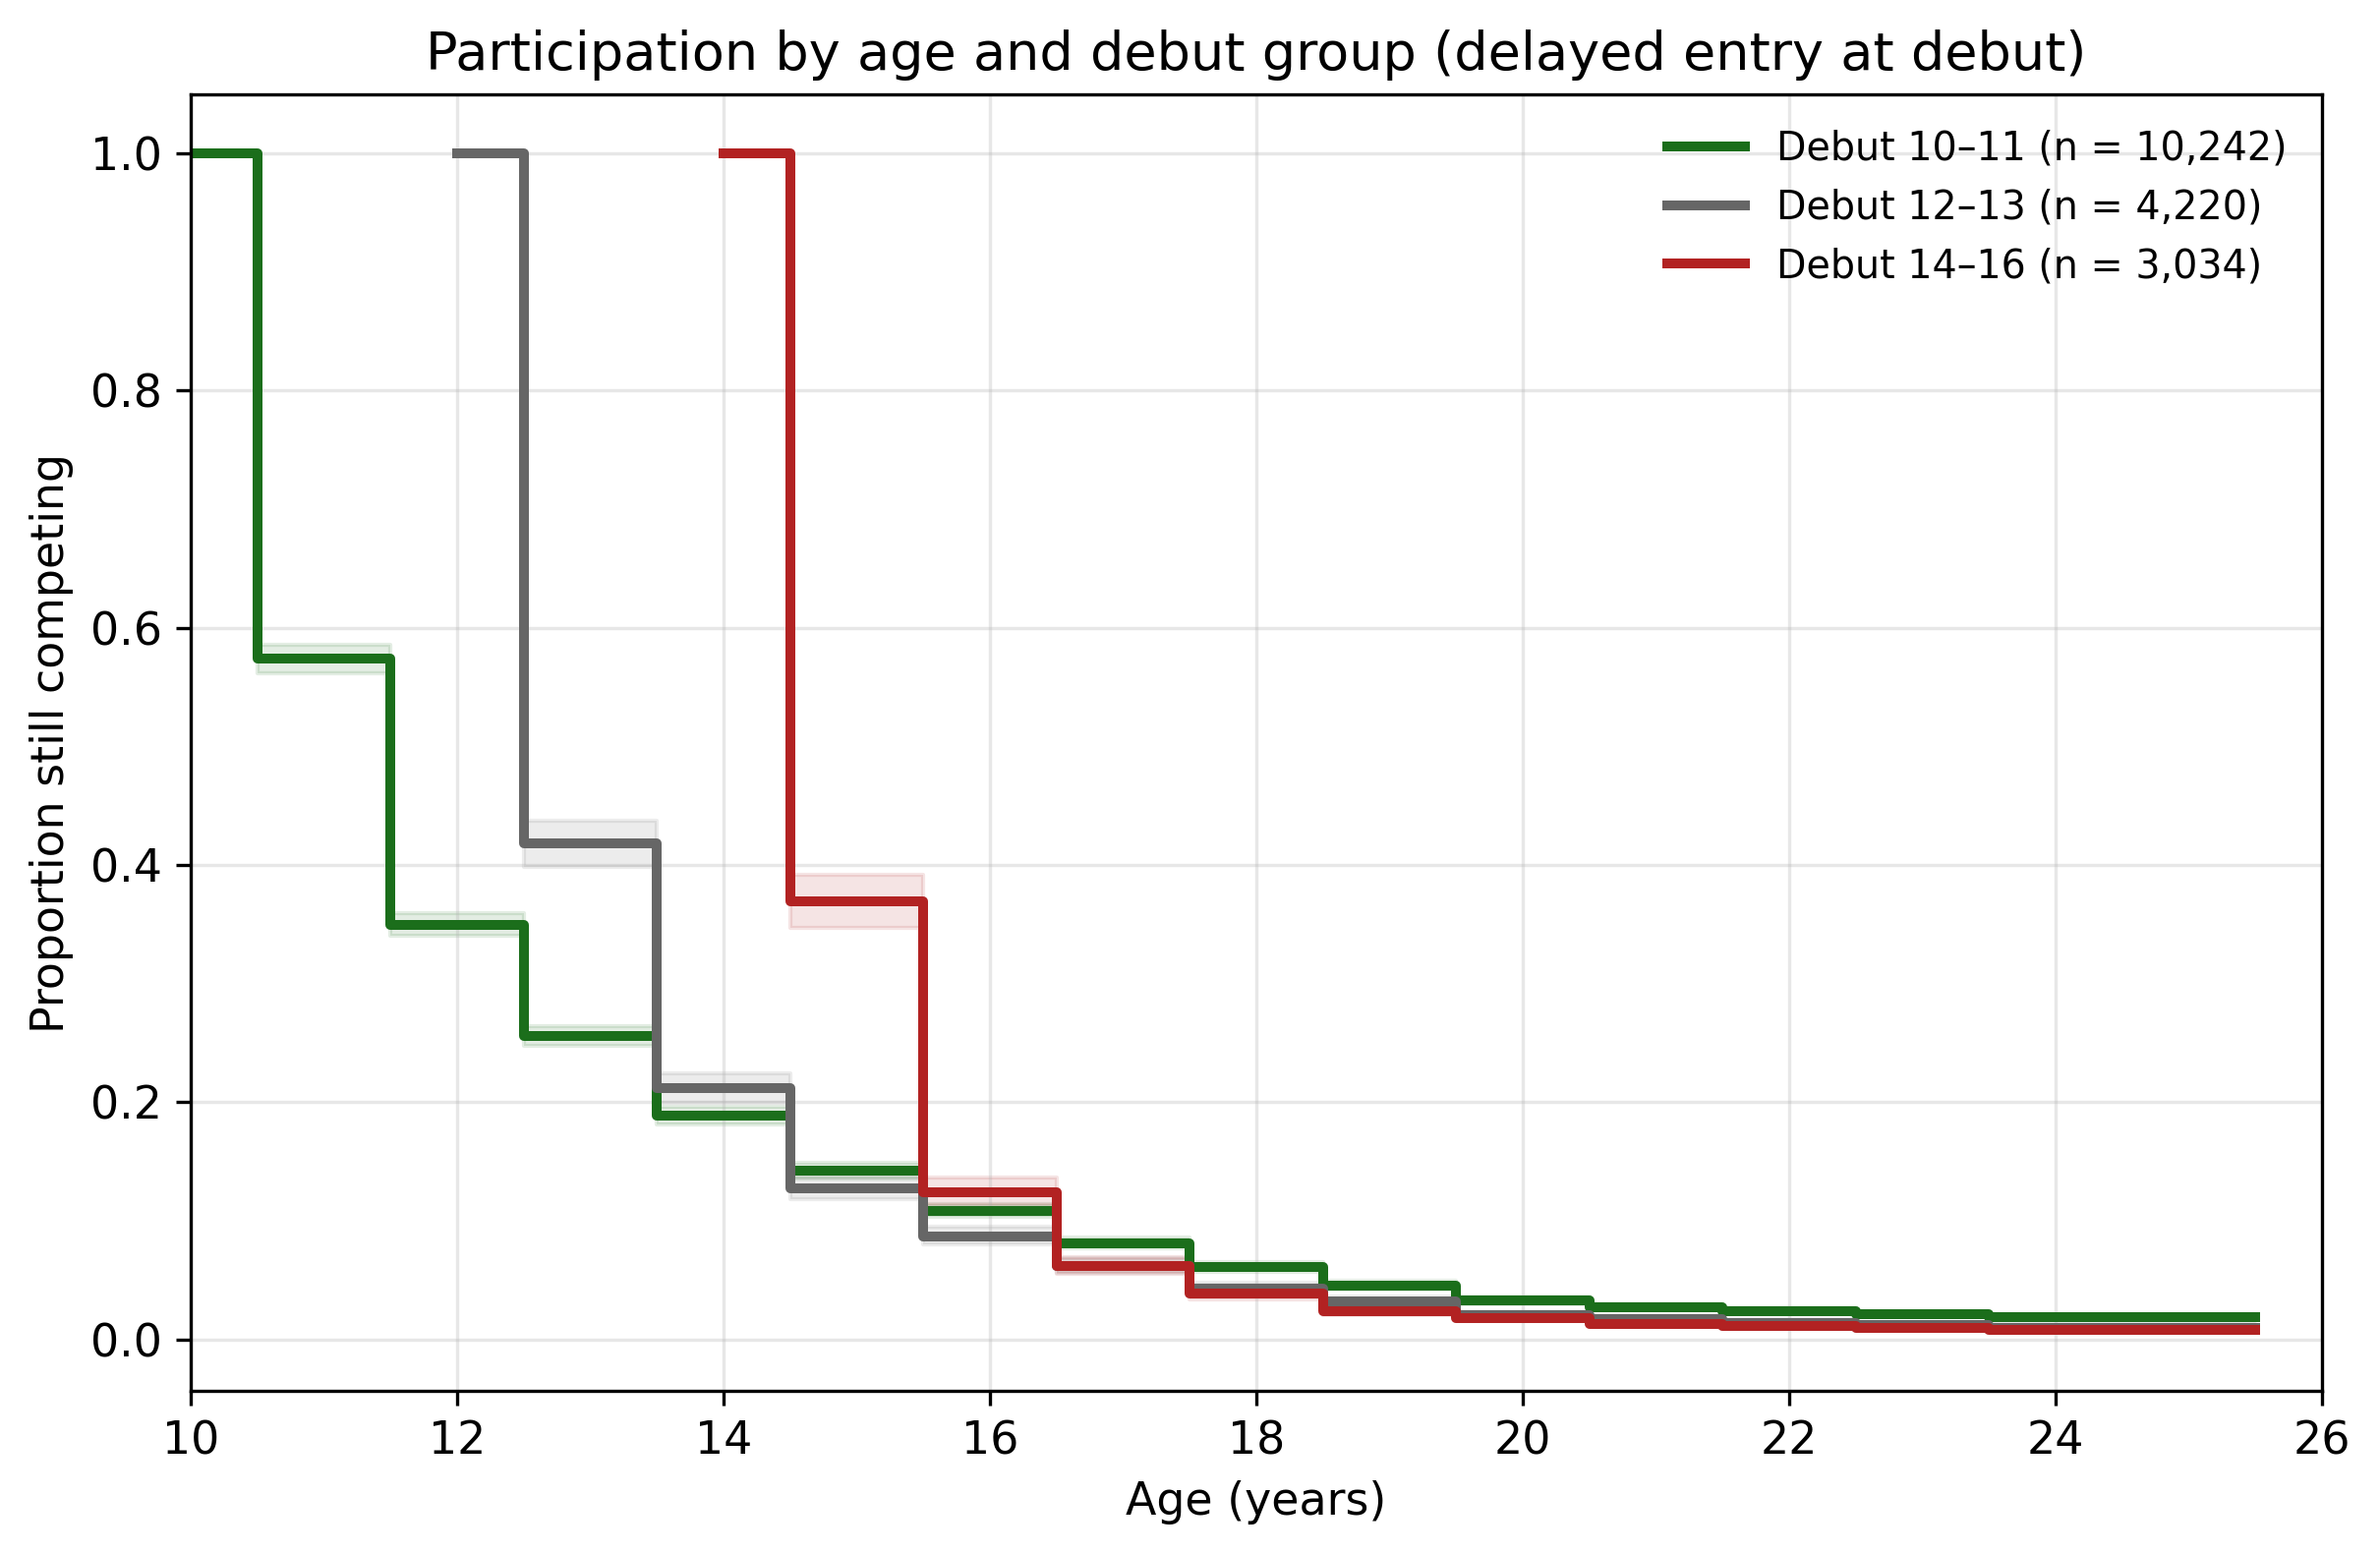
\includegraphics[width=0.9\textwidth]{fig3_km_entry.png}
\caption{Participation by age and debut group, Kaplan--Meier with delayed entry at debut (born 2001--2005). Athletes active in 2025--2026 are censored. The curves converge from about age 16.}
\label{fig:km}
\end{figure}

\begin{figure}[H]
\centering
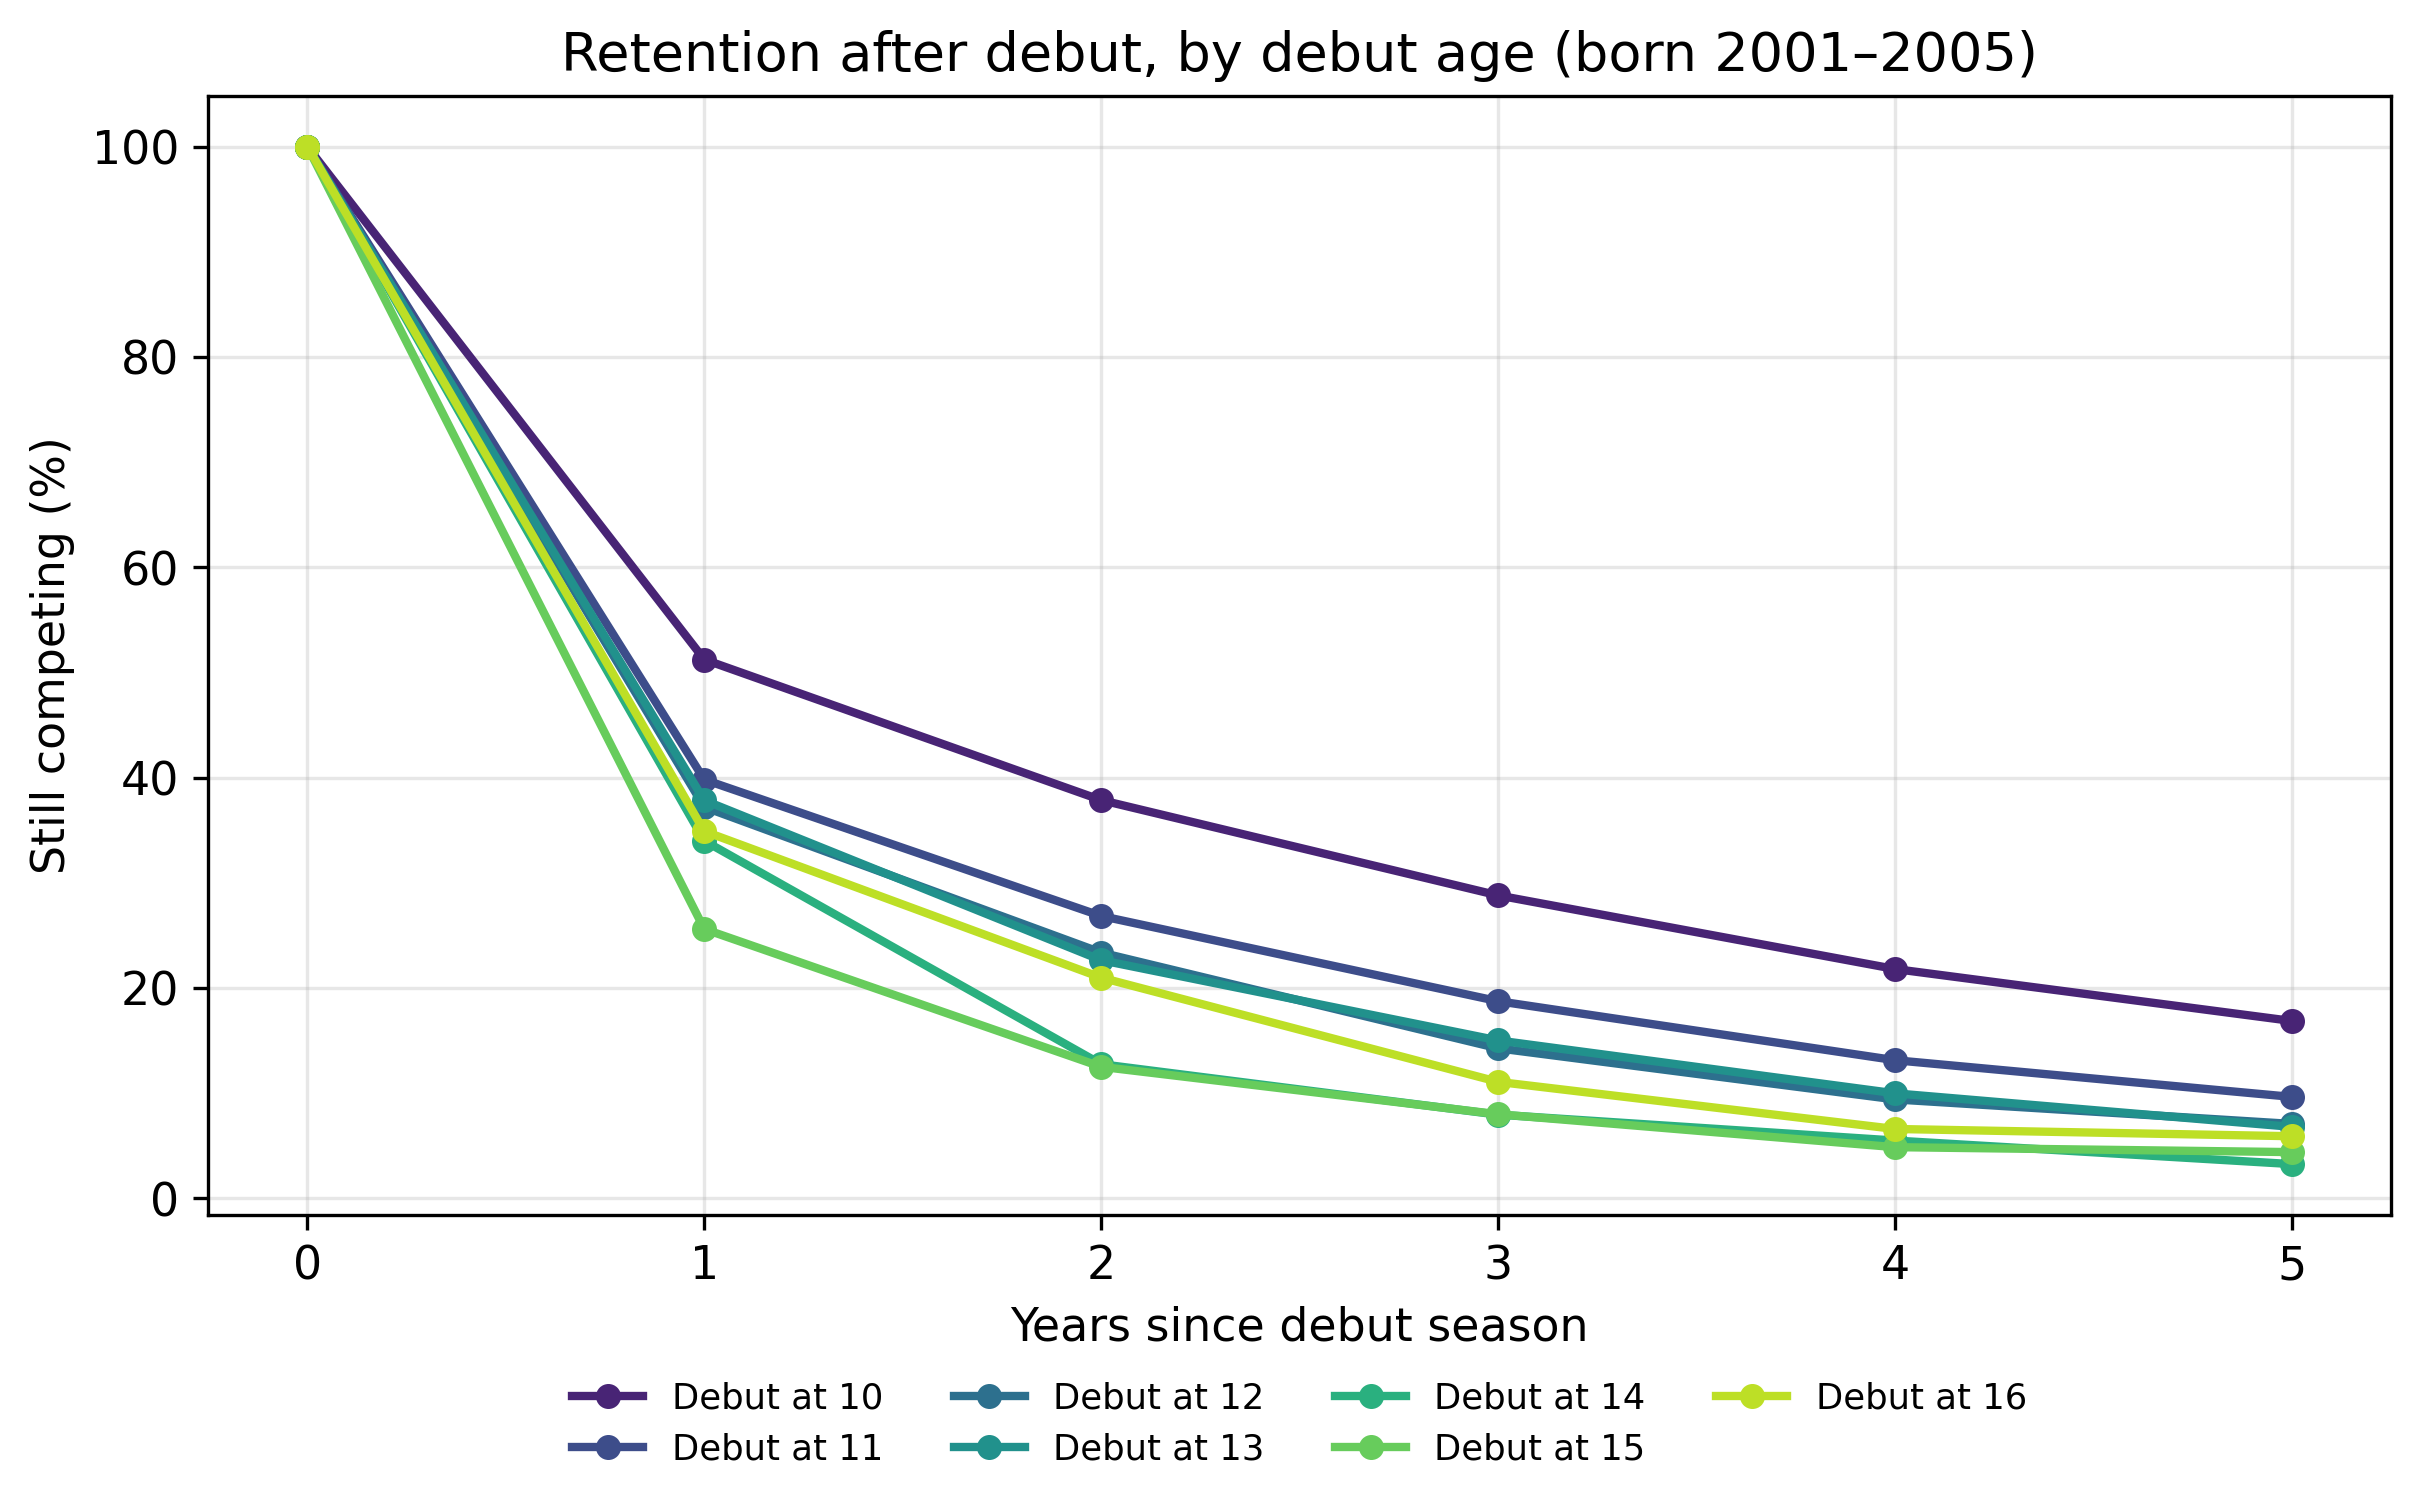
\includegraphics[width=0.85\textwidth]{fig4_retention_k.png}
\caption{Retention $k$ years after the debut season, by debut age (born 2001--2005).}
\label{fig:retk}
\end{figure}

\subsection{Among survivors, history adds nothing once current engagement is known (H3)}

Only 1\,922 of the 17\,496 debutants (11.0\,\%) were still active at age 17; 546 of these (28.4\,\%) became active seniors. In this landmark sample, earlier debut appeared protective: OR 0.87 per year of later debut (95\,\% CI 0.83--0.92). Adding current engagement --- competition days at ages 16--17 --- removed the association entirely (OR 0.97, 95\,\% CI 0.92--1.03). Conditional on having reached 17 and on how much the athlete competes now, when they started no longer carries information. This replicates, for entry history, what the companion studies found for early competition volume \cite{guttormsen2026dropout} and early performance \cite{guttormsen2026progression}: in this registry, recent behaviour dominates history.

\subsection{Robustness}

The pre-specified variations (Table~\ref{tab:robust}) altered nothing material. Excluding COVID-era debuts left the trend null (0.95, 95\,\% CI 0.90--1.01); the one-result senior outcome gave 1.00; activity at 17 among debuts at 10--14 gave 0.97; conditioning on debut-season volume gave 0.94 (95\,\% CI 0.90--1.00); the cohort halves agreed (0.98 and 0.99); and athletes debuting at 17 or older --- outside the primary range --- converted at distinctly higher rates (OR 2.46 vs.\ debut at 10, 95\,\% CI 1.49--4.08), an extension of the U's right arm consistent with strong self-selection into very late entry. The exploratory debut age $\times$ birth-quarter interaction was compatible with no modification (OR 1.04 per quarter-year, 95\,\% CI 1.00--1.09), on the selected 53\,\% of the sample with exact birth dates.

\begin{table}[H]
\centering
\caption{Robustness analyses. Estimates are for debut age (per +1 year, linear) unless stated; outcome is senior activity unless stated.}
\label{tab:robust}
\small
\begin{tabular}{lccc}
\toprule
Analysis & n & Events & OR (95\,\% CI) \\
\midrule
Primary linear trend & 17\,496 & 546 & 0.99 (0.94--1.04) \\
Excluding debuts in 2020--2021 & 17\,305 & 530 & 0.95 (0.90--1.01) \\
Outcome: $\geq$1 result at age $\geq$20 & 17\,496 & 694 & 1.00 (0.96--1.05) \\
Outcome: active at $\geq$17 (debuts 10--14) & 16\,209 & 1\,621 & 0.97 (0.93--1.00) \\
Adding debut-season competition days & 17\,496 & 546 & 0.94 (0.90--1.00) \\
Cohorts born 2001--2003 & 10\,667 & 349 & 0.98 (0.92--1.05) \\
Cohorts born 2004--2005 & 6\,829 & 197 & 0.99 (0.91--1.08) \\
Debut at 17+ vs.\ debut at 10 (categorical) & 17\,689 & 564 & 2.46 (1.49--4.08) \\
Debut age $\times$ birth quarter (exploratory) & 9\,330 & 538 & 1.04 (1.00--1.09) \\
Club-clustered robust SE (trend) & 17\,496 & 546 & 0.99 (0.93--1.04) \\
\bottomrule
\end{tabular}
\end{table}

\FloatBarrier

% ════════════════════════════════════════════════════════════
\section{Discussion}

\subsection{Principal findings}

In the complete entry population of Norwegian youth track and field, age at first competition carried no simple message about who would still be competing as an adult. Senior conversion was U-shaped --- highest for the earliest (10) and the latest (16, and 17+) entrants, lowest in between --- with a null linear trend. Measured from their own start, later entrants churned much faster, half of the ten-year-old debutants surviving the first year against a quarter to a third of teenage debutants; yet survival curves converged by about age 16, and among athletes still active at 17, entry history carried no information once current competition volume was known.

\subsection{Neither camp's prediction survives}

The early-specialisation caution, applied to competitive entry, predicts that early debutants burn out and later entrants persist \cite{difiori2014}; the early-engagement finding from football predicts the opposite \cite{vanyperen2021}. The population data support neither as stated. Early debutants did not convert worse --- they converted \emph{better} than the 11--14 entrants and were by far the most durable on the duration clock. But late entrants did not simply fail either: those who entered at 15--16, and especially 17+, converted at the highest rates of all. The resolution is selection. Entry at 10 is largely a parental and club decision made for children; entry at 16 is a decision adolescents make for themselves, and those who make it are a small, motivated group (they were also more often male, and their careers, when they failed, failed fast). The football finding that dropouts ``started later'' \cite{vanyperen2021} is consistent with our duration-clock churn --- late starters leave faster once started --- but at the level of long-run conversion, the U-shape shows that neither early nor late entry is, in itself, a liability. We note that these are associations shaped by who chooses to enter when; the registry cannot see motivation, prior training, or participation in other sports, and competition debut is not the start of sport involvement.

\subsection{The first season is the universal filter}

The dominant feature of every debut group is the first-year cliff: the median debutant competed on one day, and between half and three quarters of each entry cohort never established themselves. This matches, at the behavioural level, the entry-stage account of the registry's relative-age structure --- selection into sustained participation happens at and immediately after entry, not in adolescent talent identification \cite{guttormsen2026rae} --- and it extends it beyond birth-date composition to participation as such. Whatever determines long-term engagement, most of its action is over within a season or two of arrival, at every entry age.

\subsection{History versus current engagement, third instalment}

The landmark result completes a pattern now replicated three times in this registry with three different exposures. Early competition volume predicts senior retention, but later volume dominates it \cite{guttormsen2026dropout}. Early performance progression predicts retention, but through the most recent window \cite{guttormsen2026progression}. And entry age predicts nothing among 17-year-old survivors once current volume is in the model. For talent systems, the registry keeps returning one lesson: what an athlete is doing \emph{now} outperforms any summary of how they got there. For retention work this is encouraging --- the system need not hold athletes' histories against them --- and it cautions against entry-age heuristics in either direction.

\subsection{Strengths and limitations}

The strengths are completeness and design: a national registry with no left truncation for these cohorts, exact entry measurement for everyone who ever entered (not only later successes, the known weakness of retrospective expertise samples \cite{barth2022,gullich2025}), explicit delayed-entry survival methods, a plan committed before estimation, and internal replication across cohort halves. The limitations are equally structural. Competition debut is not sport start: children may train for years before their first meet, and late debutants may arrive from other sports with long athletic histories, so the exposure is entry into \emph{registered competition}. Exit from the registry is not exit from sport. Selection into debut age is unmeasured and surely strong; no causal reading is offered. Birth dates are missing for most brief early participants, so the birth-quarter analysis is exploratory and selected. The senior outcome is rare (3.1\,\%), so even twofold relative differences are small in absolute terms. Finally, the age-scale Cox estimate blends entry and career-stage effects, which is why the duration-aligned retention table carries the H2 conclusion.

% ════════════════════════════════════════════════════════════
\section{Perspective}

For federations and clubs, these population figures replace two competing intuitions with three usable facts. First, there is no wrong age to start: every entry age from 10 to 16 --- and beyond --- produced senior athletes, and the late-entry channel converted at the highest per-head rates, so recruitment of teenagers is worth real effort even though each teenage debutant is a short-odds, fast-resolving prospect. Second, the decisive window is the first season or two after entry, whenever entry happens: retention work should concentrate where the churn is, at the entry transition, rather than on managing entry timing. Third, by late adolescence the system should look forward, not backward: among those still competing at 17, current engagement tells the whole story and starting age tells none of it. In a federation whose teenage recruitment has halved over a decade, the finding that late entrants are disproportionately productive --- and that their main risk is simply failing to take root in the first year --- is directly actionable.

% ── Declarations ────────────────────────────────────────────

\section*{Declarations}

\noindent\textbf{Funding.} The author received no funding for this work.

\medskip\noindent\textbf{Competing interests.} The author declares no competing interests. The author maintains an open, non-commercial statistics platform built on the federation's public results database.

\medskip\noindent\textbf{Ethics.} The study analyses public competition results and falls outside the scope of the Norwegian Health Research Act; an assessment from Sikt was obtained. No individual athlete is identified. No performance data were used, and no analysis below age 13 goes beyond participation itself, in keeping with the Norwegian children's sport regulations.

\medskip\noindent\textbf{Data availability.} The underlying data are the Norwegian Athletics Federation's public competition results. Aggregate outputs and all analysis code are available from the author; athlete-level files are regenerable from the registry with the deposited code.

\medskip\noindent\textbf{Author contributions.} AGG conceived the study, performed all analyses, and wrote the manuscript.

\medskip\noindent\textbf{Declaration of AI use.} The author used a large language model (Claude, Anthropic) for programming assistance and manuscript drafting support. The author reviewed, verified, and edited all content and takes full responsibility for the integrity of the work.

\medskip\noindent\textbf{Acknowledgements.} The author thanks the Norwegian Athletics Federation, whose systematic registration of competition results makes population research of this kind possible.

% ── References ──────────────────────────────────────────────

\bibliographystyle{unsrt}
\bibliography{references}

\end{document}
